\documentclass[12pt]{article}
\usepackage{amsfonts}
\usepackage{amsthm}
\usepackage{amsmath}
\usepackage[mathscr]{euscript}
\usepackage{array}
\usepackage[thinlines]{easytable}
\usepackage{tikz}
\usepackage{pgfplots}
\usepackage[margin=2cm]{geometry}
\usepackage{graphicx}
\usepackage{xcolor}
\usepackage[utf8]{inputenc}
\usepackage[T1]{fontenc}
%\usepackage[portuguese]{babel}
\usepackage{braket}
\usepackage{thmtools} 
\usepackage{hyperref}
\usepackage{environ}
\usepackage{enumitem}
\usepackage[backend=biber, style=numeric]{biblatex} %Imports biblatex package
\addbibresource{references.bib} %Import the bibliography file
\usetikzlibrary{angles,quotes}

\usepackage{lipsum} % Pode tirar esse :D

\graphicspath{.Images/}

\hypersetup{
	colorlinks=true,
	linkcolor=blue,
	filecolor=magenta,      
	urlcolor=cyan,
	pdftitle={Quântica Avançada - L2 - Lucas Froguel}
}


\def\be{\begin{equation}}
	\def\ee{\end{equation}}
\def\bee{\begin{equation*}}
	\def\eee{\end{equation*}}
\def\bea{\begin{eqnarray*}}
	\def\eea{\end{eqnarray*}}
\def\beaa{\begin{eqnarray}}
	\def\eeaa{\end{eqnarray}}

\def\f{\frac}
\def\del{\partial}

\def\R{\mathbb{R}}
\def\K{\mathbb{K}}
\def\C{\mathbb{C}}
\def\I{\mathbb{I}}
\def\Z{\mathbb{Z}}
\def\Q{\mathbb{Q}}
\def\N{\mathbb{N}}

\def\cd{\cdot}

\def\v#1{{\boldsymbol{#1}}}
\def\ve#1{\hat{\boldsymbol#1}}

\def\l{\left}
\def\r{\right}
\def\la{\l\langle}
\def\ra{\r\rangle}
\def\div{\nabla\cdot}
\def\curl{\nabla\times}
\def\grad{\nabla}
\def\lap{\nabla^2}

\def\s{\quad}
\def\ss{\qquad}
\def\infi{\infty}
\def\p{\partial}
\def\u{\cup}%union of two sets
\def\i{\cap}%intersection of two sets
\def\ds{\oplus}



\newtheorem{exercise}{Exercise}
\newtheorem{partinner}{Part}[exercise]

\newlist{exercises}{enumerate}{1}
\setlist[exercises]{wide = 0pt, listparindent=\parindent,labelsep = 0pt,leftmargin =\labelwidth}
\setlist[exercises, 1]{label =\itshape \bfseries Part~\arabic*.\; }

\newenvironment{answer}{\noindent\textbf{\textit{Answer.}} \normalfont }{\par\noindent\rule{\textwidth}{0.4pt}}
\NewEnviron{multianswer}[1][false]{%
	\ifthenelse{\equal{#1}{true}}%
	{\def\rulewidth{\textwidth}}%
	{\def\rulewidth{0.7\textwidth}}%
	\\ \noindent\textbf{\textit{Answer.}} \normalfont%
	\BODY%
	\par\noindent\rule{\rulewidth}{0.1pt}%
}


\newcommand\norm[1]{\left\lVert#1\right\rVert}

\DeclareMathOperator{\atan}{atan}
\DeclareMathOperator{\cotan}{cotan}
\DeclareMathOperator{\acos}{acos}
\DeclareMathOperator{\sech}{sech}
\DeclareMathOperator{\csch}{csch}
\DeclareMathOperator{\asinh}{asinh}
\DeclareMathOperator{\atanh}{atanh}
\DeclareMathOperator{\acoth}{acoth}
\DeclareMathOperator{\acosh}{acosh}
\DeclareMathOperator{\acsch}{acsch}
\DeclareMathOperator{\asech}{asech}
\DeclareMathOperator{\D}{D}
\DeclareMathOperator{\tr}{tr}
\DeclareMathOperator{\Res}{Res}

\title{Mecânica Quântica Avançada \\ Lista 2}
\author{Lucas Froguel \\ IFT}
\date{}

\begin{document}
	\maketitle
	\listoftheorems[title={List of Exercises}]
	
	\begin{exercise}[6.5.1 - Independence of the tensor product from the choice of basis] \label{LM}
		Verify that the definition (6.3) of the tensor product of two vectors is independent of the choice of basis in $\mathcal{H}_1$ and $\mathcal{H}_2$.
	\end{exercise}
	\begin{answer}
		Let $\ket{n'}$ and $\ket{m'}$ be two other basis of the Hilbert spaces one and two, respectively. Then, it is true that
		\be
			\begin{aligned}
				\ket{n} &= \sum a_{n'}\ket{n'} \\
				\ket{m} &= \sum b_{m'}\ket{m'}
			\end{aligned}	
		\ee	
		Thus, we can write
		\bea
			\ket{\varphi}\otimes\ket{\chi} &=& \sum_{n, m} c_nd_m\ket{n}\otimes\ket{m} \\ 
				&=& \sum_{n, m} c_nd_m \l(\sum_{n'} a_{n'}\ket{n'}\r) \otimes \l(\sum_{m'}b_{m'}\ket{m'} \r) \\
				&=& \sum_{n', m'} a_{n'}b_{m'} \l(\sum_n c_n \r) \l(\sum_m d_m\r) \ket{n'}\otimes\ket{m'} \\
				&=& \sum_{n', m'} e_{n'} f_{m'} \ket{n'}\otimes\ket{m'}
		\eea
		This shows that the tensor product does not depend on the choice of basis.		
	\end{answer}

	\begin{exercise}[2 - Representação matricial de produtos tensoriais]
		Calculate the tensor products of two-level systems.
	\end{exercise}
	\begin{answer}
		We can calculate the tensor products of $\ket{+}$ and $\ket{-}$ as follows:
		
		\begin{align*}
			\ket{+} \otimes \ket{-} &= \begin{pmatrix} 1 \\ 0 \end{pmatrix} \otimes \begin{pmatrix} 0 \\ 1 \end{pmatrix} \\
			&= \begin{pmatrix} 1\begin{pmatrix} 0 \\ 1 \end{pmatrix} \\ 0\begin{pmatrix} 0 \\ 1 \end{pmatrix} \end{pmatrix} \\
			&= \begin{pmatrix} 0 \\ 1 \\ 0 \\ 0 \end{pmatrix} 
		\end{align*}
		
		\begin{align*}
			\ket{-} \otimes \ket{+} &= \begin{pmatrix} 0 \\ 1 \end{pmatrix} \otimes \begin{pmatrix} 1 \\ 0 \end{pmatrix} \\
			&= \begin{pmatrix} 0\begin{pmatrix} 1 \\ 0 \end{pmatrix} \\ 1\begin{pmatrix} 1 \\ 0 \end{pmatrix} \end{pmatrix} \\
			&= \begin{pmatrix} 0 \\ 0 \\ 1 \\ 0 \end{pmatrix}
		\end{align*}
		
		\begin{align*}
			\ket{-} \otimes \ket{-} &= \begin{pmatrix} 0 \\ 1 \end{pmatrix} \otimes \begin{pmatrix} 0 \\ 1 \end{pmatrix} \\
			&= \begin{pmatrix} 0\begin{pmatrix} 0 \\ 1 \end{pmatrix} \\ 1\begin{pmatrix} 0 \\ 1 \end{pmatrix} \end{pmatrix} \\
			&= \begin{pmatrix} 0 \\ 0 \\ 0 \\ 1 \end{pmatrix} 
		\end{align*}
		
		Now for the three dimension qubits, we will write the answers directly:
		\bea
			\ket{+++} &=& \begin{bmatrix} 1 \\ 0 \\ 0 \\ 0 \\ 0 \\ 0 \\ 0 \\ 0 \\ \end{bmatrix}, \qquad
			\ket{++-} = \begin{bmatrix} 0 \\ 1 \\ 0 \\ 0 \\ 0 \\ 0 \\ 0 \\ 0 \\ \end{bmatrix} \\
			\ket{+-+} &=& \begin{bmatrix} 0 \\ 0 \\ 1 \\ 0 \\ 0 \\ 0 \\ 0 \\ 0 \\ \end{bmatrix}, \qquad
			\ket{+--} = \begin{bmatrix} 0 \\ 0 \\ 0 \\ 1 \\ 0 \\ 0 \\ 0 \\ 0 \\ \end{bmatrix} \\
			\ket{-++} &=& \begin{bmatrix} 0 \\ 0 \\ 0 \\ 0 \\ 1 \\ 0 \\ 0 \\ 0 \\ \end{bmatrix}, \qquad
			\ket{-+-} = \begin{bmatrix} 0 \\ 0 \\ 0 \\ 0 \\ 0 \\ 1 \\ 0 \\ 0 \\ \end{bmatrix} \\
			\ket{--+} &=& 	\begin{bmatrix} 0 \\ 0 \\ 0 \\ 0 \\ 0 \\ 0 \\ 1 \\ 0 \\ \end{bmatrix}, \qquad
			\ket{---} = \begin{bmatrix} 0 \\ 0 \\ 0 \\ 0 \\ 0 \\ 0 \\ 0 \\ 1 \\ \end{bmatrix}
		\eea
	\end{answer}
	
	\begin{exercise}[6.5.2]
		Write down explicitly the 4$\times$4 matrix $A\otimes B$, the tensor product of the 2$\times$2 matrices $A$ and $B$:
		\be
			A = 
			\begin{pmatrix}
				a & b \\
				c & d
			\end{pmatrix}, \qquad
			B = 
			\begin{pmatrix}
				\alpha & \beta \\ 
				\gamma & \delta 
			\end{pmatrix}
		\ee
	\end{exercise}
	\begin{answer}
		It is very easy do perform this calculation:
		\be
			A \otimes B = 
			\begin{pmatrix}
				a\alpha & a\beta & b\alpha & b\beta \\
				a\gamma & a\delta & b\gamma & b\delta \\
				c\alpha & c\beta & d\alpha & d\beta \\
				c\gamma & c\delta & d\gamma & d\delta \\
			\end{pmatrix}.
		\ee
		We just multiply each element of the first matrix by the whole second matrix. 
	\end{answer}
	
	\begin{exercise}[6.5.3 - Properties of state operators]
		\begin{exercises}
			\item Show that $\rho_{ii}\geq 0$, $\rho_{jj}\geq 0$, and $\det{A} \geq 0$, from which $|\rho_{ij}|^2 \leq \rho_{ii} \rho_{jj}$ . Also deduce that if $\rho_{ii} = 0$, then $\rho_{ij} = \rho_{ji}^* = 0$.
			\begin{multianswer}
				We can always write
				\be
					\rho = \sum a_n \ket{\phi_n}\bra{\phi_n}
				\ee
				for some states $\ket{\phi_n}$ and $a_n\geq 0$. Thus, the diagonal matrix elements are
				\bea
					\rho_{ii} &=& \bra{\phi_i} \l(\sum a_n \ket{\phi_n}\bra{\phi_n}\r) \ket{\phi_i} \\
						&=& a_i 
				\eea
				Hence, $\rho_{ii}\geq0$. We also note that
				\be
					\det{A} = \rho_{ii}\rho_{jj} - |\rho_{ij}|^2
				\ee
				where we used the fact that $A$ is hermitian. This implies that
				\be
					\det{A} \geq 0 \iff |\rho_{ij}|^2 \leq \rho_{ii}\rho_{jj}
				\ee
				Using this inequality, if $\rho_{ii}=0$, then
				\be
					0 \leq \rho_{ij}\rho_{ji} \leq 0
				\ee
				Obviously, $\rho_{ij}=0$ or $\rho_{ji}=0$, but is does not matter, because they are the complex conjugate of each other, so if one is zero, the other is zero as well.				
			\end{multianswer}
			
			% Part 2
			\item Show that if there exists a maximal test giving 100$\%$ probability for the quantum state described
			by a state operator $\rho$, then this state is a pure state. Also show that if $\rho$ describes a pure state,
			and if it can be written as
			\be
				\rho = \lambda\rho' + (1 - \lambda)\rho'', 0 \leq \lambda 
				\leq 1
			\ee
			then $\rho=\rho'=\rho''$ . Hint: first demonstrate that if $\rho'$ and $\rho''$ are generic state operators, then $\rho$ is
			a state operator. The state operators form a convex subset of Hermitian operators.
			\begin{multianswer}[true]
				Let us suppose the state in which there is a probability of 1 is $\ket{\psi}$ and let $P_\psi=\ket{\psi}\bra{\psi}$. Then having a probability of one means:
				\be
					\tr\l( P_\psi\rho\r) = 1
				\ee
				In general, we could write
				\be
					\rho = \sum_i c_i \ket{\psi_i}\bra{\psi_i}
				\ee
				where we define $\psi_0\equiv\psi$. Then, if we use this definition into the expression above, we can easily see that both equations together imply
				\be
					c_0 = 1
				\ee
				However, as $\sum_i |c_i|^2 = 1$, we must have $c_i=0\ \forall\ i>0$. Hence, $\rho=\ket{\psi}\bra{\psi}$ is a pure state. We will suppose that $\rho\not=\rho'\not=\rho''$. If that is the case, then the state $\rho$ can be described as a statistical mixture of $\rho'$ (with $p=\lambda$) and $\rho''$ (with $p=1-\lambda$). As we know $\rho$ is a pure state, it is false the assertion that $\rho\not=\rho'\not=\rho''$. Thus, we prove the result asked.  
			\end{multianswer}
		\end{exercises}
	\end{exercise}
	
	\begin{exercise}[4]
		Ao ter provado o item 2 do exercício 6.5.3 do Le Bellac, você provou
		que um operador de estado $\rho$ correspondente a um estado puro não pode ser
		escrito como combinação linear de dois outros operadores de estado genéricos $\rho_1$ e $\rho_2$. Esse resultado tem a ver com a seguinte observação: "A preparação de um estado	puro é única enquanto que a preparação de um estado misto é sempre ambígua". Você poderia explicar o que uma coisa tem a ver com a outra, isto é, o que o resultado que você provou tem a ver com a preparação de um estado físico e
		possíveis resultados de medida?
	\end{exercise}
	\begin{answer}
		Dado um operador de estado puro, existe uma e apenas uma maneira de prepará-lo, que é coloca-lo no estado $\ket{\psi}\bra{\psi}$. No entanto, para um estado misto, para qualquer $\lambda\in\mathbb{R}$, sempre existirão operadores $\rho_1, \rho_2$ tais que $\rho$ seja uma combinação linear deles ponderada por $\lambda$, de modo que é impossível saber exatamente qual foi usada na preparação do estado. 
	\end{answer}

	\begin{exercise}[5]
		 Considere a seguinte matriz densidade de um spin 1/2:
		\be
			\rho = \f{1}{4}\mathbb{I} + \f{1}{2} \ket{+, \hat{a}}\bra{+, \hat{a}}
		\ee
		onde $\ket{+, \hat{a}}$ é o autoestado da projeção do operador de spin ao longo de um eixo
		a com autovalor $+\hbar/2$. Calcule a probabilidade como função de $\theta$ de encontrar o
		valor $-\hbar/2$ ao se medir o spin ao longo de um eixo b, em que $\theta$ é o ângulo entre a e b, i.e. $\hat{a}\cdot\hat{b} = \cos\theta$.
	\end{exercise}
	\begin{answer}
		Queremos calcular:
		\bea
			p(\hbar/2, \hat{b}) &=& \tr \l( \rho \ket{+, \hat{b}}\bra{+, \hat{b}}\r) \\
				&=& \f{|\braket{+, \hat{b} | +, \hat{b}}|^2}{4} + \f{|\braket{+, \hat{a} | +, \hat{b}}|^2}{2} 
 		\eea
		\begin{figure}[h!]
			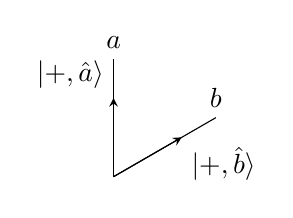
\begin{tikzpicture}[>=stealth]
				% Axes
				%\draw[->] (0,0,0) -- (2,0,0) node[below right] {$x$};
				%\draw[->] (0,0,0) -- (0,2,0) node[above] {$y$};
				% Line a
				\draw[-] (0,0,0) -- (0,1.5,0) node[above] {$a$};
				% Line b
				\draw[-] (0,0,0) -- ({1.5*cos(30)},{1.5*sin(30)},0) node[above] {$b$};		
				% Vectors
				\draw[->] (0,0,0) -- (0,1,0) node[above left] {$\ket{+, \hat{a}}$};
				\draw[->] (0,0,0) -- ({cos(30)},{sin(30)},0) node[below right] {$\ket{+, 		\hat{b}}$};
			\end{tikzpicture}
			\centering 
			\caption{The vectors $\hat{a}$ and $\hat{b}$.}
			\label{fig1}
		\end{figure}
		Precisamos, então, considerar o termo $\braket{+, \hat{a} | -, \hat{b}}$. Pela Fig(\ref{fig1}), vemos que o produto interno dos vetores pode ser escrito como $\cos\theta$, pois têm norma unitária. Portanto,
		\be
			p(+\hbar/2, \hat{b}) = \f{1}{4} + \f{\cos^2\theta}{2}
		\ee
		Como precisa ser que $p(+\hbar/2, \hat{b}) + p(-\hbar/, \hat{b}) = 1$, então vale que
		\be
			p(-\hbar/2, \hat{b}) = \f{1}{4} + \f{\sin^2\theta}{2}
		\ee
	\end{answer}

	\begin{exercise}[6]
		Considere a seguinte matriz densidade de dois spins 1/2:
		\be
			\rho = \f{\mathbb{I}}{8} + \f{1}{2} \ket{\Psi_-}\bra{\Psi_-}
		\ee
		onde $\ket{\Psi_-}$ é o estado singleto (i.e. o estado de spin total igual a zero). Suponhamos que medimos um dos spins ao longo de um eixo $a$ e o outro ao longo de um eixo $b$, em que  $\hat{a}\cdot\hat{b} = \cos\theta$. Qual é a probabilidade (como função de $\theta$) de encontramos	$+\hbar/2$ para ambos spins nestas medidas?
	\end{exercise}
	\begin{answer}
		O estado de singleto é 
		\be
			\ket{\Psi_-} = \f{\ket{+-} - \ket{-+}}{\sqrt{2}}
		\ee
		Portanto,
		\be
			\rho = \f{1}{8}\mathbb{I} + \f{1}{4}\l( \ket{+-}\bra{+-} - \ket{+-}\bra{-+} - \ket{-+}\bra{+-} + \ket{-+}\bra{-+} \r)
		\ee
		O estado que queremos medir é
		\be
			\ket{\phi} = \ket{+}_a\ket{+}_b
		\ee
		onde o índice significa o eixo em relação ao qual estamos considerando. Sejam $\theta_a$ e $\theta_b$ os ângulos que os eixos $a$ e $b$ fazem com o eixo $z$. Então,
		\bea
			\ket{+}_a &=& \cos(\theta_a/2)\ket{+} + \sin(\theta_a/2)\ket{-} \\
			\ket{+}_b &=& \cos(\theta_b/2)\ket{+} + \sin(\theta_b/2)\ket{-} 
		\eea
		O projetor que projeta no estado desejado é $P_\phi = \ket{\phi}\bra{\phi}$. Ou seja,
		\bea
			\ket{\phi} &=& \l(\cos(\theta_a/2)\ket{+} + \sin(\theta_a/2)\ket{-} \r)\l( \cos(\theta_b/2)\ket{+} + \sin(\theta_b/2)\ket{-} \r) \\
				&=& \cos\f{\theta_a}{2}\cos\f{\theta_b}{2}\ket{+}\ket{+} + \cos\f{\theta_a}{2}\sin\f{\theta_b}{2}\ket{+}\ket{-} + \sin\f{\theta_a}{2}\cos\f{\theta_b}{2}\ket{-}\ket{+} + \sin\f{\theta_a}{2}\sin\f{\theta_b}{2}\ket{-}\ket{-}
		\eea
		Portanto, o operador é
		\begin{align*}
			P_\phi &= \ket{\phi}\bra{\phi} \\
			&= \left(\cos\frac{\theta_a}{2}\cos\frac{\theta_b}{2}\ket{+}\ket{+} + \cos\frac{\theta_a}{2}\sin\frac{\theta_b}{2}\ket{+}\ket{-} + \sin\frac{\theta_a}{2}\cos\frac{\theta_b}{2}\ket{-}\ket{+} + \sin\frac{\theta_a}{2}\sin\frac{\theta_b}{2}\ket{-}\ket{-}\right) \\
			&\times \left(\cos\frac{\theta_a}{2}\cos\frac{\theta_b}{2}\bra{+}\bra{+} + \cos\frac{\theta_a}{2}\sin\frac{\theta_b}{2}\bra{+}\bra{-} + \sin\frac{\theta_a}{2}\cos\frac{\theta_b}{2}\bra{-}\bra{+} + \sin\frac{\theta_a}{2}\sin\frac{\theta_b}{2}\bra{-}\bra{-}\right) \\
			&= 	 \cos^2\frac{\theta_a}{2}\cos^2\frac{\theta_b}{2}\ket{+}\ket{+}\bra{+}\bra{+} + \sin^2\frac{\theta_a}{2}\sin^2\frac{\theta_b}{2}\ket{-}\ket{-}\bra{-}\bra{-} + \\
			&\quad
			\cos^2\frac{\theta_a}{2}\sin^2\frac{\theta_b}{2}\ket{+}\ket{-}\bra{+}\bra{-} 
			+ \sin^2\frac{\theta_a}{2}\cos^2\frac{\theta_b}{2}\ket{-}\ket{+}\bra{-}\bra{+} + \\
			&\quad \cos\f{\theta_a}{2}\sin\f{\theta_b}{2}\sin\f{\theta_a}{2}\cos\f{\theta_b}{2} \ket{+}\ket{-}\bra{-}\bra{+} + \cos\f{\theta_a}{2}\sin\f{\theta_b}{2}\sin\f{\theta_a}{2}\cos\f{\theta_b}{2} \ket{-}\ket{+}\bra{+}\bra{-} + \cdots
		\end{align*}
		Os termos omitidos são aqueles que não aparecem em $\rho$, de modo que serão zero ao se tomar o traço de $P_\phi\rho$. Vamos, então, calcular a probabilidade
		\bea
			p_{++} &=& \tr\l( P_\phi\rho\r) \\
				&=& \f{1}{8}\l( \cos^2\frac{\theta_a}{2}\cos^2\frac{\theta_b}{2} + \sin^2\frac{\theta_a}{2}\sin^2\frac{\theta_b}{2} + 
				\cos^2\frac{\theta_a}{2}\sin^2\frac{\theta_b}{2} + \sin^2\frac{\theta_a}{2}\cos^2\frac{\theta_b}{2} \r) + \\
				&\quad& \f{1}{4}\l( \cos^2\f{\theta_a}{2}\sin^2\f{\theta_b}{2} - \sin\f{\theta_a}{2}\cos\f{\theta_a}{2}\sin\f{\theta_b}{2}\cos\f{\theta_b}{2} - \sin\f{\theta_a}{2}\cos\f{\theta_a}{2}\sin\f{\theta_b}{2}\cos\f{\theta_b}{2} + \sin^2\frac{\theta_a}{2}\cos^2\frac{\theta_b}{2} \r) \\
				&=& \f{1}{8} + \f{1}{4}\l( \cos\f{\theta_a}{2}\sin\f{\theta_b}{2} - \sin\f{\theta_a}{2}\cos\f{\theta_b}{2} \r)^2 \\
				&=& \f{1}{8} + \f{1}{4}\sin^2\l(\f{\theta_b - \theta_a}{2}\r)
		\eea
		Ora, é fácil ver que $\theta=|\theta_b-\theta_a|$. Como o seno ao quadrado é uma função par, $\sin^2\theta = \sin^2(-\theta)$. Portanto, podemos escrever
		\be
			p_{++} = \f{1}{8} + \f{1}{4}\sin^2\l(\f{\theta}{2}\r)
		\ee
	\end{answer}
	
	\begin{exercise}[7]
		Considere um sistema bipartite descrito por um operador de estado
		$\rho^{AB}$ que evolui unitariamente:
		\be\label{ML}
			i\hbar\f{d\rho^{AB}}{dt} = \l[ H_{AB}, \rho_{AB} \r]
		\ee
		com $H_{AB} = H_A + H_B + V_{AB}$ onde $H_A$ depende somente das coordenadas do subsistema $A$, $H_B$ depende somente das coordenadas do subsistema $B$ e $V_{AB}$ depende das coordenadas de ambos subsistemas. Mostre que o operador de densidade reduzido do sistema $A$, i.e.
		$\rho^{A} = \tr_B(\rho^{AB})$, obedece à seguinte equação de evolução temporal:
		\be
			i\hbar\f{d\rho^A}{dt} = \l[ H_A, \rho^A\r] + \tr_B\l[V_{AB}, \rho^{AB}\r]
		\ee
		Você acabou de mostrar que enquanto o sistema bipartite evolui unitariamente, o subsistema A não evolui unitariamente em geral. No curso de Física Estatística você, muito provavelmente, vai provar esse resultado novamente.
	\end{exercise}
	\begin{answer}
		Vamos aplicar o traço em $B$ na Eq.(\ref{ML}) e deduzir a expressão que queremos. Obviamente, o lado esquerdo trivialmente dá a expressão que queremos, então focaremos no lado direito. Considere
		\bea
			\tr_B \l[ H_{AB}, \rho_{AB} \r] &=& \tr_B(H_{AB}\rho^{AB}) - \tr_B(\rho^{AB}H_{AB}) \\
				&=& \tr_B\l( H_A\rho^{AB} + H_B\rho^{AB} + V_{AB}\rho^{AB}  \r) - \tr_B\l( \rho^{AB}H_A + \rho^{AB}H_B \rho^{AB}V_{AB}   \r) \\
				&=& \l( H_A\tr_B(\rho^{AB}) - \tr_B(\rho^{AB})H_A \r) +  \tr_B\l( V_{AB}\rho^{AB} - \rho^{AB}V_{AB} \r) + \l( \tr_B(H_B\rho^{AB}) - \tr_B(\rho^{AB}H_B)  \r) \\
				&=& [H_A, \rho_A] + \tr_B[V_{AB}, \rho^{AB}]
		\eea
		* Como o último termo se anula? 
		Portanto, juntando as duas pontas:
		\be
			i\hbar\f{d\rho^A}{dt} = \l[ H_A, \rho^A\r] + \tr_B\l[V_{AB}, \rho^{AB}\r]
		\ee
	\end{answer}
	
	\begin{exercise}[8]
		Mostre que sob evolução unitária (ou hamiltoniana, i.e. quando o
		operador densidade evolui de acordo com a Eq. (6.37) do Le Bellac) a entropia de	emaranhamento é conservada no tempo.
	\end{exercise}
	\begin{answer}
		A evolução unitária é dada por
		\be
			i\hbar\f{d\rho}{dt} = \l[ H, \rho \r]
		\ee
		E a entropia de emaranhamento é
		\be
			S = -\tr(\rho\ln\rho)
		\ee
		Logo,
		\bea
			\f{dS}{dt} &=& -\f{d}{dt}\tr(\rho\ln\rho) \\
				&=& - \tr\l( \dot{\rho} + \dot{\rho}\ln\rho \r) \\
				&=& -\tr(\dot{\rho}(1+\ln\rho)) \\
				&=& -\f{1}{i\hbar} \tr\big( (H\rho-\rho H)(1+\ln\rho) \big) \\
				&=& -\f{1}{i\hbar} \tr\big( H\rho + H\rho\ln\rho - \rho H - \rho H\ln\rho \big) \\
				&=& - \f{1}{i\hbar}\tr\big( [H, \rho] + [H\rho, \rho] \big)
		\eea
		* terminar 
	\end{answer}

	\begin{exercise}[9]
		Considere os estados de Bell.
		\bea
			\ket{\Phi_+} &=& \f{1}{\sqrt{2}} (\ket{++} + \ket{--}) \\
			\ket{\Phi_-} &=& \f{1}{\sqrt{2}} (\ket{++} - \ket{--}) \\
			\ket{\Psi_+} &=& \f{1}{\sqrt{2}} (\ket{+-} + \ket{-+}) \\
			\ket{\Psi_-} &=& \f{1}{\sqrt{2}} (\ket{+-} - \ket{-+}) \\
		\eea
		\begin{exercises}
			\item Escreva os estados de Bell e as correspondentes matrizes densidade na forma
			matricial na representação definida pela Eq. (1).
			\begin{multianswer}
				Pelo Ex.(\ref{LM}), já sabemos as formas matriciais de cada um dos elementos da base. Basta realizar as somas/subtrações correspondentes.
				\bea
					\ket{\Phi_+} = \f{1}{\sqrt{2}}
					\begin{pmatrix} 1 \\ 0 \\ 0 \\ 1 \end{pmatrix}, 
					&\quad& 
					\ket{\Phi_-} = \f{1}{\sqrt{2}}
					\begin{pmatrix} 1 \\ 0 \\ 0 \\ -1 \end{pmatrix} \\
					\ket{\Psi_+} = \f{1}{\sqrt{2}}
					\begin{pmatrix} 0 \\ 1 \\ 1 \\ 0 \end{pmatrix}, 
					&\quad& 
					\ket{\Psi_-} = \f{1}{\sqrt{2}}
					\begin{pmatrix} 0 \\ 1 \\ -1 \\ 0 \end{pmatrix}
				\eea
				Já as matrizes de densidade são apenas os produtos $\rho=\ket{\psi}\bra{\psi}$. 
				\bea
					\rho(\Phi_+) &=& \ket{\Phi_+}\bra{\Phi_+} 
						= \f{1}{2} 
						\begin{pmatrix} 1 \\ 0 \\ 0 \\ 1 \end{pmatrix}
						\begin{pmatrix} 1 & 0 & 0 & 1 \end{pmatrix} 
						= \f{1}{2}
						\begin{pmatrix}
							1 & 0 & 0 & 1 \\
							0 & 0 & 0 & 0 \\
							0 & 0 & 0 & 0 \\
							1 & 0 & 0 & 1 \\
						\end{pmatrix} \\
					\rho(\Phi_-) &=& \ket{\Phi_-}\bra{\Phi_-} 
					= \f{1}{2} 
					\begin{pmatrix} 1 \\ 0 \\ 0 \\ -1 \end{pmatrix}
					\begin{pmatrix} 1 & 0 & 0 & -1 \end{pmatrix} 
					= \f{1}{2}
					\begin{pmatrix}
						1 & 0 & 0 & -1 \\
						0 & 0 & 0 & 0 \\
						0 & 0 & 0 & 0 \\
						-1 & 0 & 0 & 1 \\
					\end{pmatrix} \\
					\rho(\Psi_+) &=& \ket{\Psi_+}\bra{\Psi_+} 
					= \f{1}{2} 
					\begin{pmatrix} 0 \\ 1 \\ 1 \\ 0 \end{pmatrix}
					\begin{pmatrix} 0 & 1 & 1 & 0 \end{pmatrix} 
					= \f{1}{2}
					\begin{pmatrix}
						0 & 0 & 0 & 0 \\
						0 & 1 & 1 & 0 \\
						0 & 1 & 1 & 0 \\
						0 & 0 & 0 & 0 \\
					\end{pmatrix} \\
					\rho(\Psi_-) &=& \ket{\Psi_-}\bra{\Psi_-} 
					= \f{1}{2} 
					\begin{pmatrix} 0 \\ 1 \\ -1 \\ 0 \end{pmatrix}
					\begin{pmatrix} 0 & 1 & -1 & 0 \end{pmatrix} 
					= \f{1}{2}
					\begin{pmatrix}
						0 & 0 & 0 & 0 \\
						0 & 1 & -1 & 0 \\
						0 & -1 & 1 & 0 \\
						0 & 0 & 0 & 0 \\
					\end{pmatrix}
				\eea
				É fácil ver que todas possuem traço 1, como deveriam.
			\end{multianswer}
			
			% Part 2
			\item Mostre que estes estados são maximamente emaranhados (ou desordenados),
			isto é, as entropias de emaranhamento correspondentes aos spins individuais assumem o valor máximo $\ln 2$.
			\begin{multianswer}[true]
				* como calcular a entropia sem usar a decomposição de Schmidt? tem como?
			\end{multianswer}
			
		\end{exercises}
	\end{exercise}
	
	\begin{exercise}[10]
		Considere o seguinte vetor de estado de dois spins 1/2 :
		\be
			\ket{\Psi(1, 2)} = \cos\theta\ket{+-} - \sin\theta\ket{-+}	
		\ee
		onde $0\leq\theta\leq\pi/2$. Obtenha a matriz densidade reduzida de um dos spins e calcule a correspondente entropia de emaranhamento. Para que valor de $\theta$ essa entropia é máxima?
	\end{exercise}
	\begin{answer}
		A matriz de densidade é:
		\bea
			\rho &=& \ket{\Psi(1, 2)}\bra{\Psi(1, 2)} \\ 
				&=& \cos^2\theta\ket{+-}\bra{+-} - \sin\theta\cos\theta\ket{+-}\bra{-+} - \sin\theta\cos\theta\ket{-+}\bra{+-} + \sin^2\theta\ket{-+}\bra{-+}
		\eea
		Isso gera uma matriz $4\times 4$. Vamos considerar a seguinte ordenação dos vetores de base $\{ \ket{++}, \ket{+-},\\ \ket{-+}, \ket{--}\}$. 
		\be
			\rho = 
			\begin{pmatrix}
				0 & 0 & 0 & 0 \\
				0 & \cos^2\theta & -\sin\theta\cos\theta & 0 \\
				0 & -\sin\theta\cos\theta & \sin^2\theta & 0 \\
				0 & 0 & 0 & 0 \\
			\end{pmatrix}
		\ee
		Obviamente, o emaranhamento é máximo para $\theta=\pi/4$, pois essa escolha não favorece nenhum estado e gera uma matriz de Bell ($\rho(\Psi_-)$, em particular). 
		* como calcular a entropia geral?
	\end{answer}
	
	\begin{exercise}[6.5.4 - ]
		Positronium is an electron–positron bound state very similar to the electron–proton bound state of the hydrogen atom.
		\begin{exercises}
			\item Calculate the energy of the ground state of positronium as a function of that of the hydrogen atom. We recall that the positron mass is equal to the electron mass.
			\begin{multianswer}
				We recall that the groundstate energy of the hydrogen atom is
				\be
					E_0 = \f{m_ee^4}{8h^2\varepsilon_0^2}
				\ee
			\end{multianswer}
			
			
		\end{exercises}
	\end{exercise}
	
	\begin{exercise}[12]
		
	\end{exercise}
	\begin{answer}
		
	\end{answer}

\end{document}